\documentclass[a4paper,10pt]{article}
%\documentclass[preview=false]{standalone}
% %%%% Define new conditional \ifplastex
% %%%% This ensure that the file complied normally without plasTeX.
\usepackage{plastex}

\ifplastex\else
\usepackage{standalone} %%%% Only load standalone when not in plasTeX
\standalonetrue
\fi

% % Package for typesetting URLs
\usepackage{url}

\usepackage{import}

\usepackage{iumlb}

\usepackage{multirow}
 
 % Package for including figures
\usepackage{graphicx}

% Package for sub-floats (e.g. figures)
\usepackage{subfig}

% % Title
\title{iUML-B User Manual} 

% % Author
\author{Colin Snook\\University of Southampton}

% % Date
\date{%
  Version 0.0.1\\%
  \today%
}

\begin{document}
\ifplastex%
\maketitle% Make title if in plasTeX mode.
\else%
 \ifstandalone%
 \maketitle % Make title if in standalone mode.
 \else%
 \fi%
\fi%

This section covers general facilities and concepts available for all iUML-B diagrams.

\section{Introduction}
\label{sec:iumlb-introduction}

iUML-B provides a diagrammatic modelling notation for Event-B in the form of state-machines and class-diagrams. The diagrammatic elements are contained within an Event-B model and generate or contribute to parts of it. For example a state-machine will automatically generate the Event-B data elements (sets, constants, axioms, variables, and invariants) to implement the states, and contribute additional guards and actions to existing events. iUML-B Class diagrams provide a way to visually model data relationships.  Classes, attributes and associations are linked to Event-B data elements (carrier sets, constants, or variables) and generate constraints on those elements.  In iUML-B class diagrams, a class represents some set of instances and the class may be used to show relationships with other classes. Usually the set of instances is given by an Event-B data element, but in some scenarios it is useful to construct a set using an expression as the class name.


%\iUMLB~\cite{said15:umlbSosym,snook14:iumlbStatem,snook06umlbTosem} provides a diagrammatic modelling notation for \eventB including state-machines and class diagrams. The diagrammatic models are contained within an \eventB machine and generate or contribute to parts of it. For example a state-machine will automatically generate the \eventB data elements (sets, constants, axioms, variables, and invariants) to implement the states while \eventB events are expected to already exist to represent the transitions. Transitions contribute further guards and actions representing their state change, to the events that they elaborate. An existing \EventB set may be associated with the state-machine to define its instances. In this case the state-machine is `lifted' so that it has a value for every instance of the associated set. State-machines are typically refined by adding nested state-machines to states.
%
%Class diagrams provide a way to visually model data relationships. Classes, attributes and associations are linked to \EventB data elements (carrier set, constant, or variable) and generate constraints on those elements. For the \VLAN we use class diagrams extensively to model the sets of entities and their relationships and we use state-machines to constrain the sequences of events and to declare state dependant invariant properties.
%\begin{figure}[!t]
%	\centering
%	\subfloat[Class diagram]{
%		\includegraphics[width=0.5\textwidth]{figures/iumlb-CD}
%		\label{fig:iumlb-cd}
%	}
%	\hspace{2em}
%	\subfloat[State-machine]{
%		\includegraphics[width=0.3\textwidth]{figures/iumlb-SM}
%		\label{fig:iumlb-sm}
%	}
%	\caption{Example \iUMLB diagrams}
%	\label{fig:iumlb}
%\end{figure}
%
%
%Figure~\ref{fig:iumlb} shows an abstract example of an \iUMLB model to illustrate the features we have used in the VLAN. We give the corresponding translation into \EventB in Figure~\ref{fig:eventb-translation}.  In Figure~\ref{fig:iumlb-cd}, there are three classes; \BCLSi, \BCLSii, which elaborate carrier sets, and \BCLSiii, which is a sub-class of \BCLSi and elaborates a variable.  An \emph{attribute} or \emph{association} of a class can have a combination of the following properties: \emph{surjective}, \emph{injective}, \emph{total}, and \emph{functional}.  Attributes \Battri of \BCLSi and \Battriii of \BCLSiii are total and functional, while \Battrii of \BCLSii is functional. An injective association \Brel defined between \BCLSi and \BCLSii elaborates a constant. Figure~\ref{fig:iumlb-sm} shows an example of a state-machine, which is lifted to the carrier set \BCLSi for its instances.  % (This is done in the diagram's properties view which is not shown).
%This is also the instances set for the class \BCLSi and a state of the state-machine is named after its variable sub-class, \BCLSiii. Further sub-states \BSi and \BSii are modelled as variable subsets of \BCLSiii. The state of an instance is represented by its membership of these sets. The state-machine transitions are linked to the same events as the methods of \BCLSiii. Hence the state-machine constrains the invocation of class methods for a particular instance of the class. The contextual instance is modelled as a parameter \BthisCLSiii which can be used in additional guards and actions in both the class diagram and the state-machine.
%\begin{figure}[!t]
%	\centering
%	\begin{Bcode}
%		{
%			{$\carriersets{\BCLSi, \BCLSii}$ \Bhspace $\constants{\Battri, \Battrii, \Brel}$} 
%			\Bhspace
%			{$\axioms{
%					{\Brel \in{} \BCLSi \pinj{} \BCLSii}
%					\Bvspace	{\Battri \in{} \BCLSi \tfun{} \nat{}}
%					\Bvspace	{\Battrii \in{} \BCLSii \tfun{} \intg{}}	
%				}$} 
%		}\Bvspace 
%		$\variables{ 
%			\Bvspace {\BCLSiii,}
%			\Bvspace {\BSi,} 
%			\Bvspace {\BSii}
%			\Bvspace {\Battriii}
%		} $ \Bhspace 
%		$\invariants{
%			{\BCLSiii \subseteq \BCLSi} \Bvspace
%			{\BSi \subseteq \BCLSiii}  \Bvspace
%			{\BSii \subseteq \BCLSiii}  \Bvspace
%			{ partition(\BCLSiii, \BSi, \BSii)} \Bvspace
%			{\Battriii \in \BCLSiii \tfun BOOL} \Bvspace
%			{ \forall{}\BthisCLSiii\qdot{}(\BthisCLSiii \in{} \BSii) \limp{}} \Bvspace
%			{~~~ (\Battriii(\BthisCLSiii) = FALSE)  }
%		}$ \Bhspace
%		$\event{INITIALISATION}{}{}{}{}{
%			{\BCLSiii  \bcmeq  \emptyset{}} \Bvspace 
%			{\BSi  \bcmeq  \emptyset{}} \Bvspace 
%			{\BSii  \bcmeq  \emptyset{}} \Bvspace 
%			{\Battriii  \bcmeq  \emptyset{}} \Bvspace 
%		}$ \Bvspace
%		$\event{\Bc}{} {\BthisCLSii , \BthisCLSiii} {
%			{\BthisCLSii \in \BCLSii}
%			\Bvspace	{\BthisCLSiii \notin \BCLSiii}
%			\Bvspace	{\Brel(\BthisCLSiii) = \BthisCLSii}
%		}{}{
%			{\BSi \bcmeq \BSi \bunion{} \{ \BthisCLSiii \}} 
%			\Bvspace 	{\BCLSiii \bcmeq \BCLSiii \bunion{} \{ \BthisCLSiii \}}
%			\Bvspace 	{\Battriii \bcmeq{} \Battriii \ovl{} \{\BthisCLSiii\mapsto{}FALSE\}}
%		}$ 
%		\Bhspace
%		$\event{\Be}{} {\BthisCLSiii , \Bb}{
%			{\BthisCLSiii \in \BCLSiii}
%			\Bvspace 	{\BthisCLSiii \in \BSi}
%			\Bvspace 	{\Bb \in{} BOOL}
%			\Bvspace	{\Battrii(\Brel(\BthisCLSiii)) > 0}
%		}{}{
%			{\BSi \bcmeq{} \BSi \setminus{} \{\BthisCLSiii\}}
%			\Bvspace	{\BSii \bcmeq{} \BSii \bunion{} \{\BthisCLSiii\}}
%			\Bvspace	{\Battriii(\BthisCLSiii) \bcmeq{} \Bb}
%		}$ 
%		%  \Bhspace $\event{\Bf}{}{}{\BSM = \BSII}{}{\BSM \bcmeq \BSMNULL}$
%	\end{Bcode}  
%	\caption{Event-B translation of the iUML-B example}
%	\label{fig:eventb-translation}
%\end{figure}
%
%The transition \Bc, from the initial state to \BSi also enters parent state \BCLSiii and therefore represents a constructor for the class \BCLSiii. The class method \Bc is also defined as a constructor  and automatically generates an action to initialise the instance of \Battriii with its defined initial value. The same event \Bc is also given as a method of class \BCLSii in order to generate a contextual instance \BthisCLSii which is used in an additional (manually entered) guard to define a value for the association \Brel of the super-class. The transition and method \Be is a normal method of class \BCLSiii, which is available when the contextual instance exists in \BCLSiii and \BSi, and changes state by moving the instance from \BSi to \BSii. The other guards and actions shown in this event concerning parameter \Bb and attribute \Battrii, have been added as additional guards and actions of the transition or method. These are not shown in the diagram as they are entered using the diagram's properties view. The state invariant shown in state \BSii applies to any instance while it is in that state. The \EventB version of the invariant is quantified over all instances and an antecedent added to represent the membership of \BSii. In the rest of this paper we do not explain the translation to \EventB.  

%\begin{figure}[!htbp]
%  \centering
%  \includegraphics[width=0.6\textwidth]{figures/iumlb-SM}
%  \caption{An example \iUMLB state-machine \Bmch{SM}}
%  \label{fig:iumlb-sm}
%\end{figure}
%Here we show a translation of state-machine \Bmch{SM} using the \emph{enumeration} encoding, where each state is encoded as a constant from an enumerated set \BSMSTATES.  Variable \BSM, which represents the current state of the state-machine, is initialised to \BSI. Events \Be and \Bf change the value of \BSM according to the transitions in the state-machine.  The Event-B translation can be seen below.



%\begin{Bcode}
%%  $\carriersets{\BSMSTATES}$ \Bhspace $\constants{\BSMNULL, \BSI, \BSII}$ \Bvspace
%%  $\axioms{\partition(\BSMSTATES, \BSMNULL, \BSI, \BSII)}$ \Bvspace 
%  $\variables{ \Bvrb{CLS3}, \Bvrb{S1}, \Bvrb{S2}}$ \Bhspace $\invariants{\BSM \in \BSMSTATES}$ \Bvspace
%  $\event{INITIALISATION}{}{}{}{}{\BSM \bcmeq \BSI}$ \Bhspace
%  $\event{\Be}{}{}{\BSM = \BSI}{}{\BSM \bcmeq \BSII}$ \Bhspace
%  $\event{\Bf}{}{}{\BSM = \BSII}{}{\BSM \bcmeq \BSMNULL}$
%\end{Bcode}

%%% Local Variables: 
%%% mode: latex
%%% TeX-master: "VLANTAG_NASA17"
%%% End: 


%\subsection{Tooling}\

The iUML-B tooling consists of a collection of plug-ins for the Rodin toolset. 
The plug-ins provide several different kinds of modelling diagrams, which enables diagrammatic models to be added as an extension to an Event-B machine. 
A translator is provided to generate Event-B elements in the machine that implements the behaviour expressed in the iUML-B diagrams. 
Hence the iUML-B model contributes additional variables, invariants, guards and actions to the existing Event-B model and its events.
As Rodin is an Eclipse based tool, so is iUML-B. 
The iUML-B  tooling is based on the Event-B EMF framework, Event-B EMF Extensions and Generic Diagrams plug-ins.


\section{Getting Started}
\label{sec:iumlb-gettingstarted}

Since iUML-B diagrams are contained within Event-B machines, start by creating an Event-B project containing a Machine project. 
Then select the machine in the Event-B navigator and right click to use the context manual. 
The context manual contains commands to add the various kinds of iUML-B diagram to the machine.

Once the machine contains a diagram, it will appear in the Event-B navigator as an element within the machine.
To open the diagram for editing, double click on the iUML-B element in the Event-B navigator.

You can now use the diagram editor palette to create new elements on the canvas. 
Use the properties sheet to edit the detailed properties of an element.
Refer to the diagram specific user manuals within this manual.

Once the diagram model has been entered, the toolbar buttons can be used to process it.
The validate button (tick icon) runs a diagram validation test to check that the diagram is well-formed.
This validation is also performed automatically before you generate from the diagram.
To generate Event-B use the translate button (UML-B icon). 
The rules for generation of Event-B are given in the diagram specific manuals.

There is also a command (`Translate All iUML-B Diagrams') in the context manual of the machine (right click the machine in the Event-B navigator).
This translates all of the iUML-B diagrams contained in the machine.

\begin{figure}[!htbp]
	\centering
	\ifplastex
	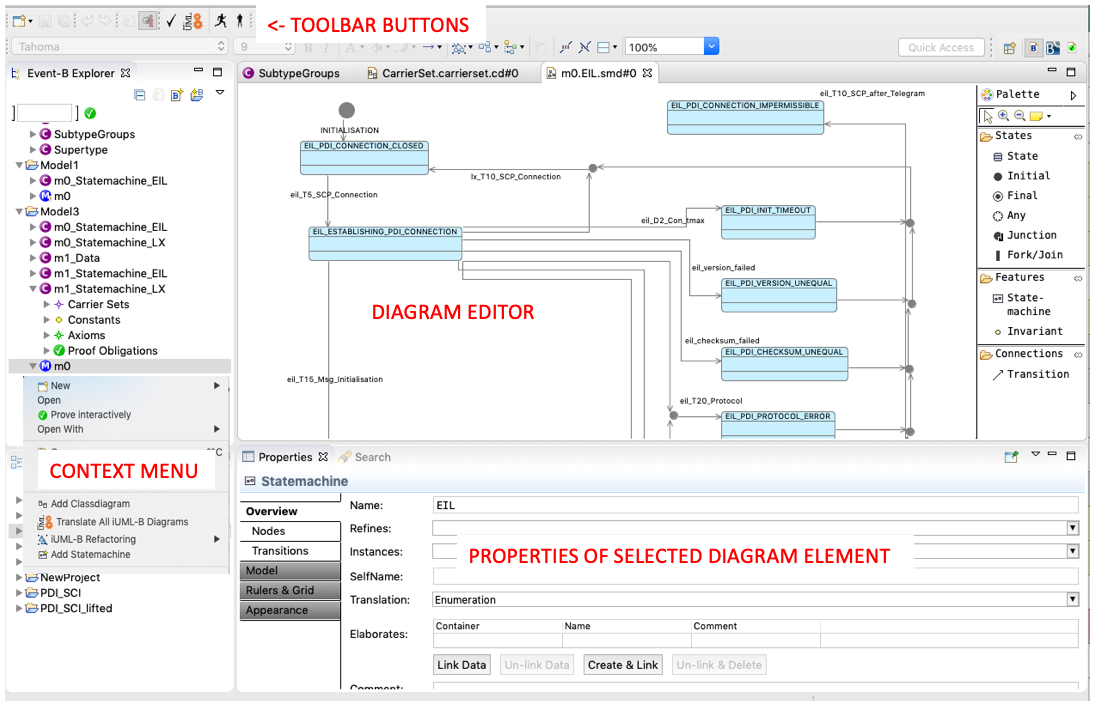
\includegraphics[width=1000]{figures/UMLB_UI.png}
	\else
	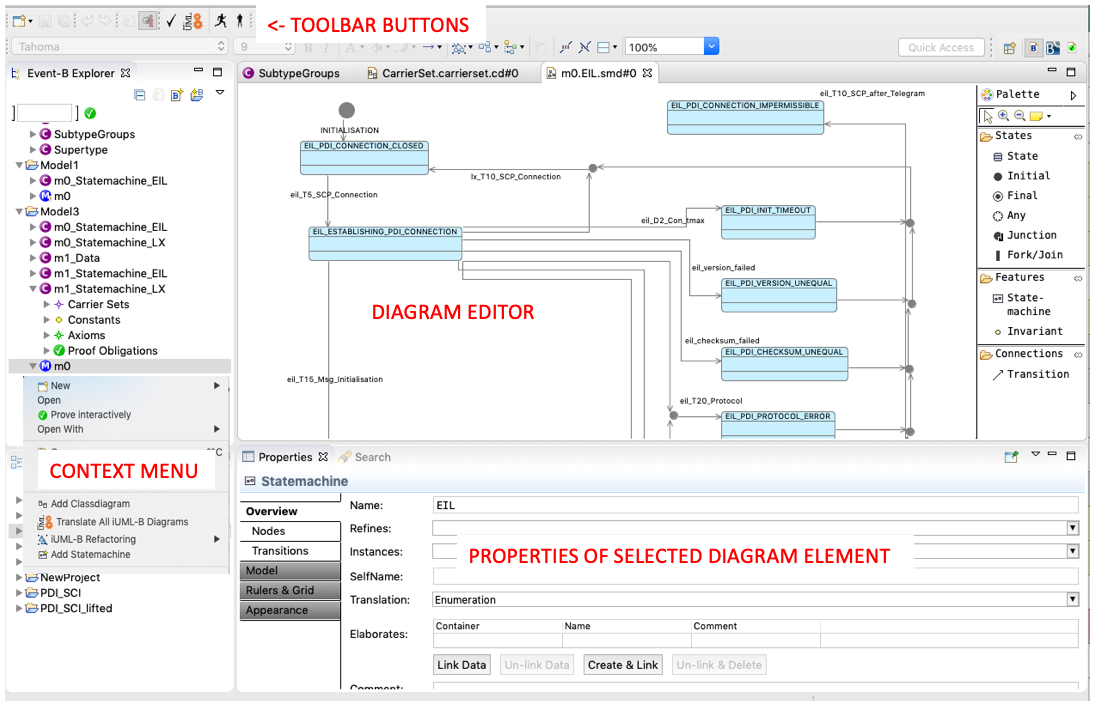
\includegraphics[width=1\textwidth]{figures/UMLB_UI.png}
	\fi
	\caption{User Interface for iUML-B}
	\label{fig:UMLB_UI}
\end{figure}

\section{Concepts}
\label{sec:iumlb-concepts}

The iUML-B diagrams generate Event-B which is annotated as generated.
The generated Event-B is read-only and editors (should) not allow you to edit it.
You can however, add manually entered elements to the Event-B machine alongside the generated ones.
The intention is to allow users both options: modelling by diagram, modelling in Event-B.

As well as generating new Event-B elements, iUML-B often \emph{elaborates} existing Event-B elements.
In the latter case, the iUML-B model element contributes to the definition or children of the elaborated element.
For example, an invariant could be generated to constrain the elaborated element.



%\input{iuml-b-tasks}
%
%\input{iuml-b-reference}
%
%\section{Refactoring}
\label{sec:component_diagrams-refactoring}

A refactoring facility is provided in iUML-B that allows a set of changes made to the collection of iUML-B diagrams in an abstract model to be propagated down the refinement chain as part of a commit action. Alternatively, the set of changes can be reverted, restoring the model to its pre-change state.
Changes cannot be committed (hence propagated) when a lower refinement also has uncommitted changes. I.e. if several refinements have uncommitted changes they must be committed or reverted in order starting from the most refined level and working up the refinement chain. 
Changes are only propagated to a refinement when they are still relevant to the refinement. Changes may have already been made in the refinement, as part of the refinement process, that mean that a subsequent change in the abstract model cannot be propagated. For example the parent element of a changed attribute may have been removed and replaced with a different model element or a guards predicate may have been edited to utilise new variables introduced in the refinement. Changes to Event-B formula attributes (i.e. predicates and actions) are only propagated when the equivalent refined formula is unchanged except for formatting (whitespace).

\subsection{Enabling Refactoring}

The refactoring facility may be enabled or disabled in the iUML-B preferences menu (Figure \ref{fig:PreferenceForEnablingRefactoring}). The current default is DISABLED.  
WARNING: If this preference is disabled while there are outstanding, uncommitted changes, and the associated model is then edited without refactoring being enabled, those change records will become invalid and wont be able to be propagated at a later stage.

 \begin{figure}[!htbp]
  \centering
  \ifplastex
  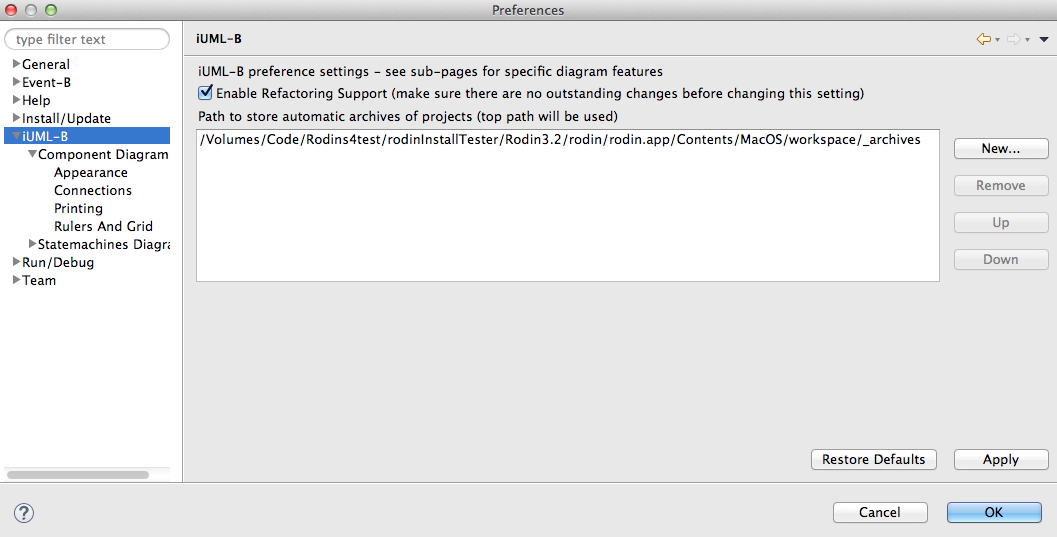
\includegraphics[width=1024]{figures/image59.png}
  \else
  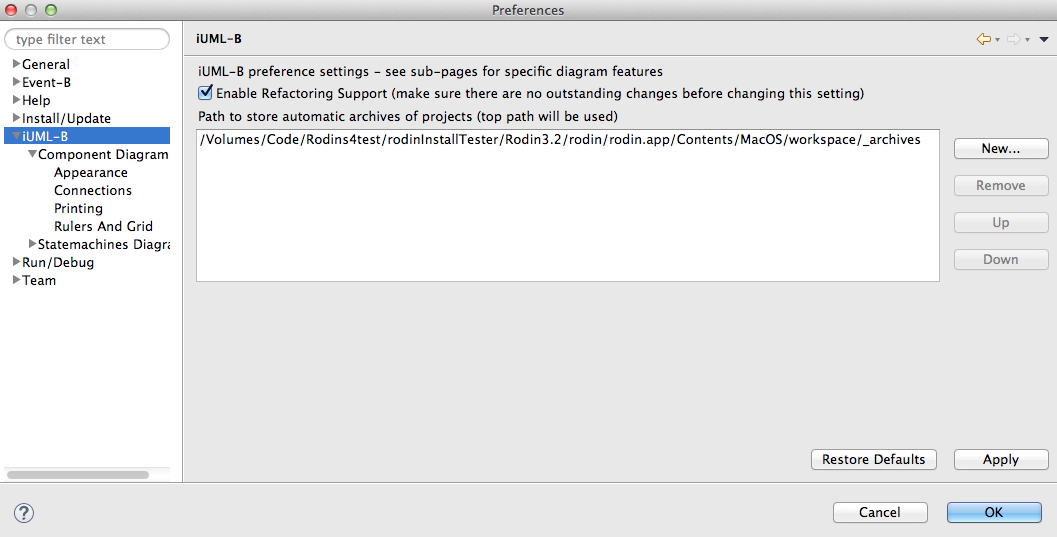
\includegraphics[width=1\textwidth]{figures/image59.png}
  \fi
  \caption{Preference for Enabling Refactoring}
  \label{fig:PreferenceForEnablingRefactoring}
\end{figure} 

\subsection{Automatic Archiving}

An archive of the complete project including any change records and reports is made before a commit is attempted. This is in case an unexpected event such as power failure should cause the commit to fail leaving the model in a corrupted state. In this case the project should be deleted and restored from the archive using the standard Eclipse import facility (\textbf{\texttt{Import - General - Existing Projects into Workspace - Select archive file}}).

\subsection{Decorator}

Machines with outstanding, uncommitted changes are decorated in the Event-B Explorer (Figure \ref{fig:DecoratorIndicatingOutstandingRecordedChanges}). 

 \begin{figure}[!htbp]
  \centering
  \ifplastex
  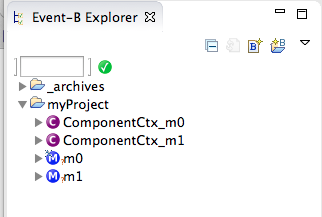
\includegraphics[width=1024]{figures/image60.png}
  \else
  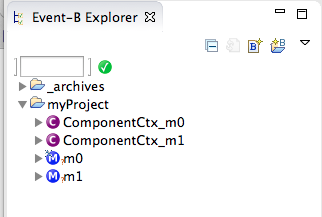
\includegraphics[width=1\textwidth]{figures/image60.png}
  \fi
  \caption{Decorator Indicating Outstanding Recorded Changes (see M0)}
  \label{fig:DecoratorIndicatingOutstandingRecordedChanges}
\end{figure} 

\subsection{Refactoring Menu: Commit and Revert}

The Commit and Revert actions are accessed from a pop-up context menu, by right clicking on a machine that has outstanding uncommitted changes (Figure \ref{fig:ContextMenuForCommitRevert}).

 \begin{figure}[!htbp]
  \centering
  \ifplastex
  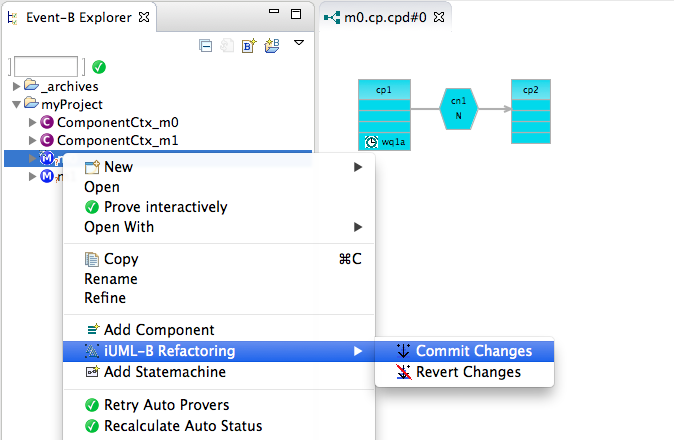
\includegraphics[width=1024]{figures/image61.png}
  \else
  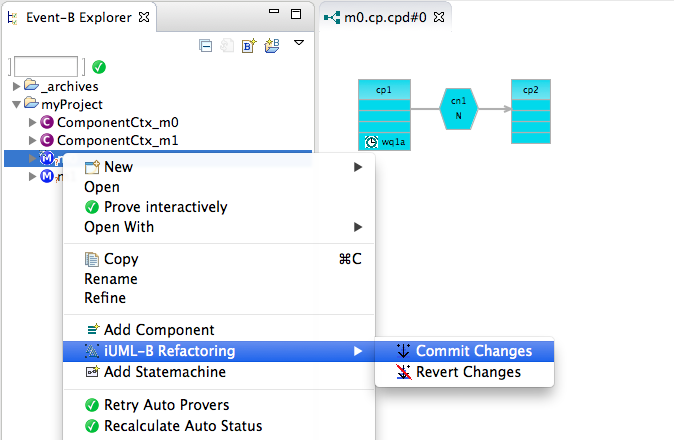
\includegraphics[width=1\textwidth]{figures/image61.png}
  \fi
  \caption{Context Menu for Commit/Revert}
  \label{fig:ContextMenuForCommitRevert}
\end{figure} 

\textbf{Commit} -
When Commit is selected for a machine that has outstanding uncommitted changes, firstly an information and confirmation message appears (Figure \ref{fig:CommitConfirmationMessage}). This gives the user a chance to cancel since the Commit operation is a significant process that can only be reversed by restoring from archive.

 \begin{figure}[!htbp]
  \centering
  \ifplastex
  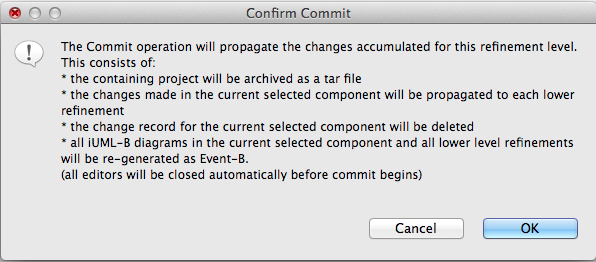
\includegraphics[width=1024]{figures/image62.png}
  \else
  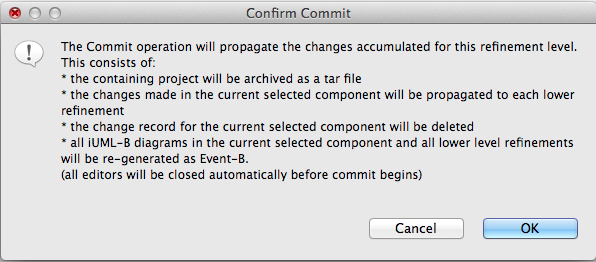
\includegraphics[width=1\textwidth]{figures/image62.png}
  \fi
  \caption{Commit Confirmation Message}
  \label{fig:CommitConfirmationMessage}
\end{figure} 

If ok is selected on Mi, the following steps will be taken
\begin{enumerate}
\item any open diagrams will be closed, 
\item the project will be archived,
\item the recorded changes for Mi will be propagated to the next level refinement Mi+1 (if any),
\item the changes made to the refinement Mi+1 will be recorded,
\item the previous change records for Mi will be deleted,
\item all diagrams of the previous model Mi will be generated,
\item steps 3 to 6 will be repeated for the refinement Mi+1,
\item a report of the complete process will be saved.
\end{enumerate}


\textbf{Revert} -
When Revert is selected for a machine that has outstanding uncommitted changes, firstly an information message appears (Figure \ref{fig:RevertConfirmationMessage}). This gives the user a chance to cancel since the Revert operation is a significant process that cannot be reversed.

 \begin{figure}[!htbp]
  \centering
  \ifplastex
  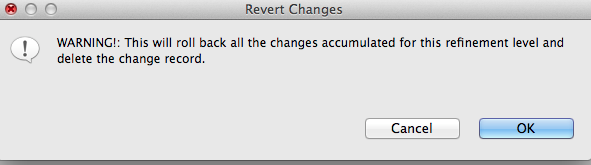
\includegraphics[width=1024]{figures/image63.png}
  \else
  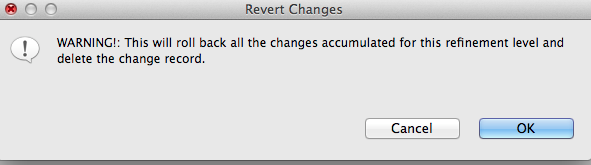
\includegraphics[width=1\textwidth]{figures/image63.png}
  \fi
  \caption{Revert Confirmation Message}
  \label{fig:RevertConfirmationMessage}
\end{figure} 

If ok is selected on a machine Mi, the following steps will be taken
\begin{enumerate}
\item any open diagrams will be closed,
\item the changes made to Mi will be reverted taking the model back to its original state,
\item the change records for Mi will be deleted,
\item all diagrams of Mi will be generated.
\end{enumerate}


\textbf{No Changes} - 
If Commit or Revert are selected for a machine that has no recorded changes, an appropriate message is displayed (Figure \ref{No Changes Error Message})and no further action is taken.

 \begin{figure}[!htbp]
  \centering
  \ifplastex
  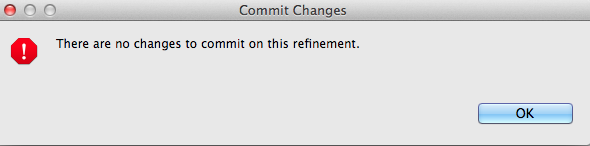
\includegraphics[width=1024]{figures/image64.png}
  \else
  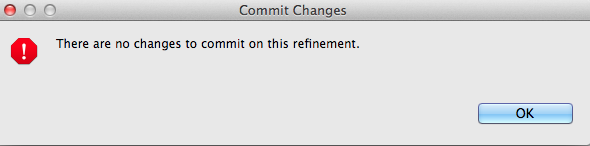
\includegraphics[width=1\textwidth]{figures/image64.png}
  \fi
  \caption{No Changes Error Message}
  \label{fig:NoChangesErrorMessage}
\end{figure} 

\subsection{Resources: Change Records and Reporting}

Various resources are created to support refactoring. In normal use it is not necessary to access these resources and they are not visible in the Event-B Explorer by default. If it is wished to examine the generated reports or the change records they can be viewed either by opening a standard Eclipse workspace file navigator or Project Explorer (using Window-Show View) or by un-selecting the All files and folders filter of the Event-B Explorer. (The second method is shown in Figure \ref{fig:RemovingAllFilesAndFoldersFilterForEventBExplorer}).

 \begin{figure}[!htbp]
  \centering
  \ifplastex
  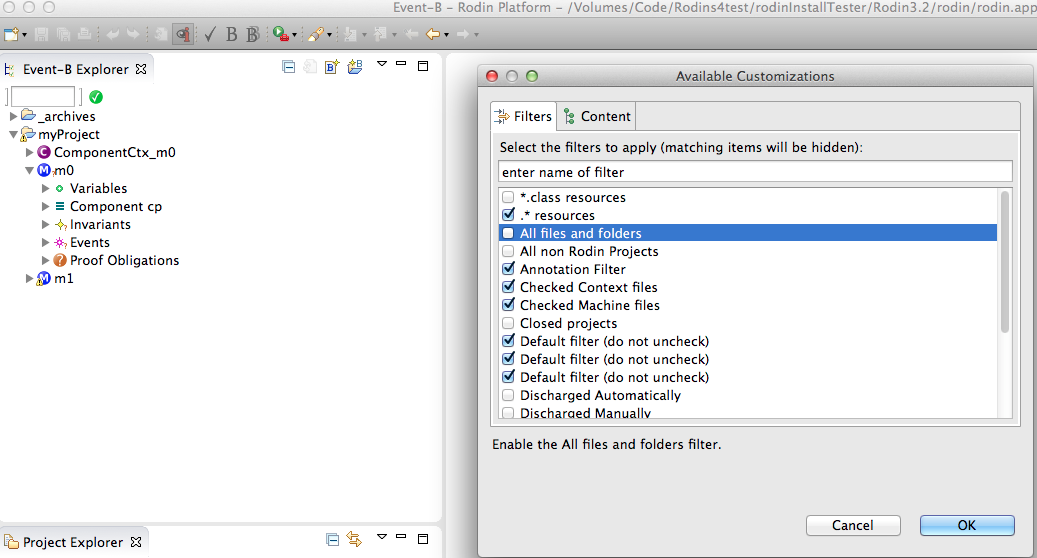
\includegraphics[width=1024]{figures/image65.png}
  \else
  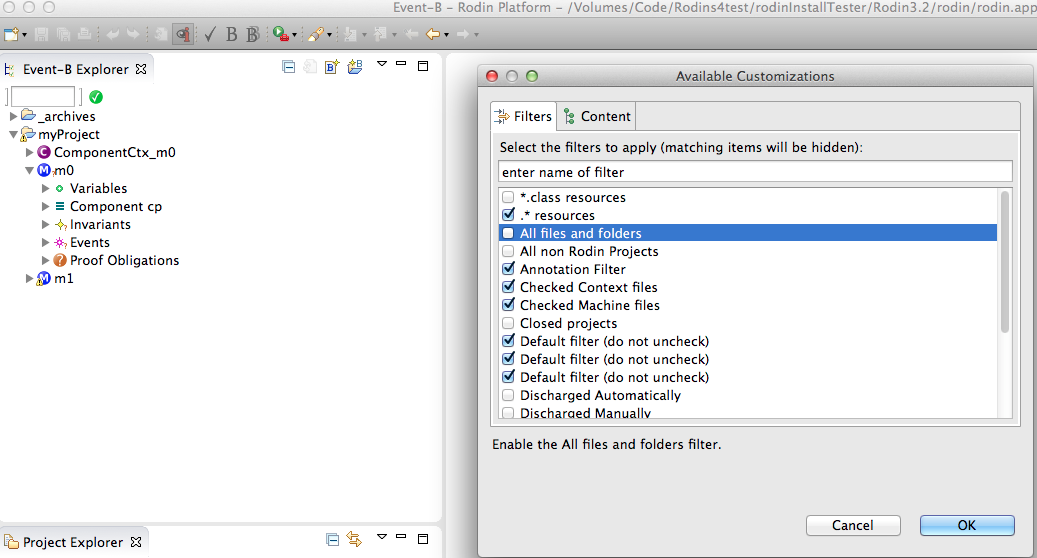
\includegraphics[width=1\textwidth]{figures/image65.png}
  \fi
  \caption{Removing `All files and folders' Filter for Event-B Explorer}
  \label{fig:RemovingAllFilesAndFoldersFilterForEventBExplorer}
\end{figure} 

The various resources that are generated (Figure \ref{fig:ChangesResourcesProducedForRefactoring}) are as follows. 
As soon as a supported editor is opened two files will appear in a folder called /iumlb/changes/ within the project. These are:
$<$myMachine$>$\_bum.xmb  -  a copy of the pre-change state of the model,
$<$myMachine$>$\_bum.equivmap - a map from the elements in the xmb file to the corresponding elements in the Rodin  model. 
These files can be opened for examination but if they are edited the refactoring process is likely to fail. The xmb file can be opened with an EMF editor such as Rose. The equivmap file can be opened with a normal text editor.
As soon as some changes to the diagram are saved a change record will appear in the same folder, $<$myMachine$>$\_bum.changes.  Again, the file can be opened with an EMF editor such as Rose but any alterations are likely to cause the refactoring process to fail.

 \begin{figure}[!htbp]
  \centering
  \ifplastex
  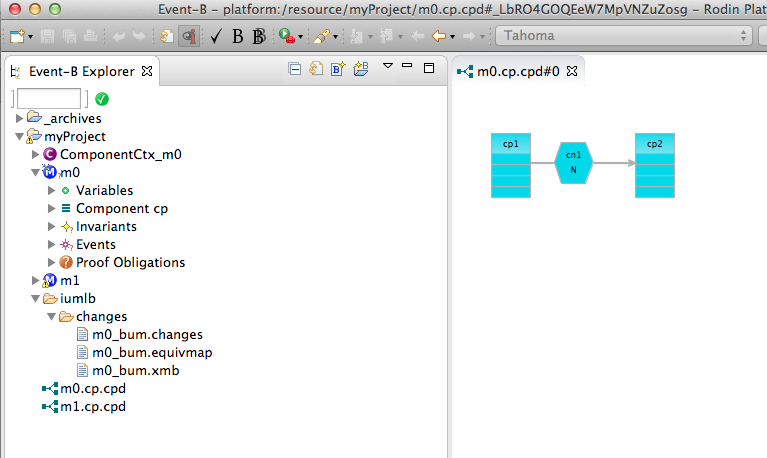
\includegraphics[width=1024]{figures/image66.png}
  \else
  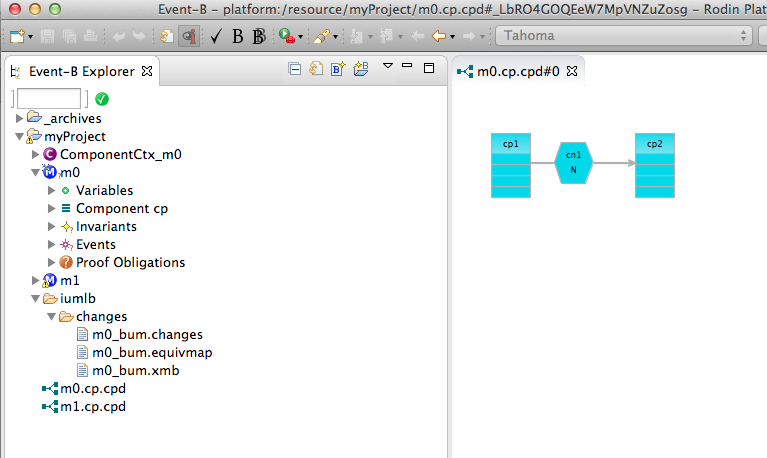
\includegraphics[width=1\textwidth]{figures/image66.png}
  \fi
  \caption{Changes Resources Produced for Refactoring}
  \label{fig:ChangesResourcesProducedForRefactoring}
\end{figure} 

Note: If these three files are deleted the project will be left in its current state with no record of changes. This can be useful if for some reason it is wished to neither commit nor revert the changes but to leave the models as they are with the abstract model edited but the changes not propagated. 
If the changes are reverted, once the revert process has completed, these three files are deleted.
If the changes are committed, once the commit has completed, these three files are deleted and a file $<$myMachine$>$\_bum.$<$timestamp$>$.report is created in the folder /iumlb/reports/. This is a text file giving a detailed record of the changes made down the refinement chain (Figure \ref{fig:ReportsProducedByRefactoring}).

 \begin{figure}[!htbp]
  \centering
  \ifplastex
  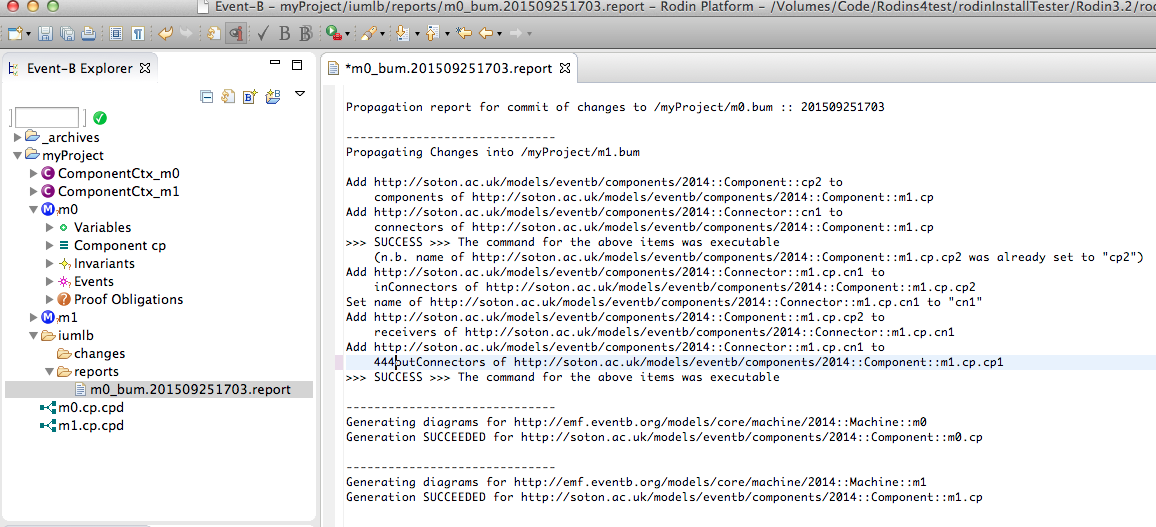
\includegraphics[width=1024]{figures/image67.png}
  \else
  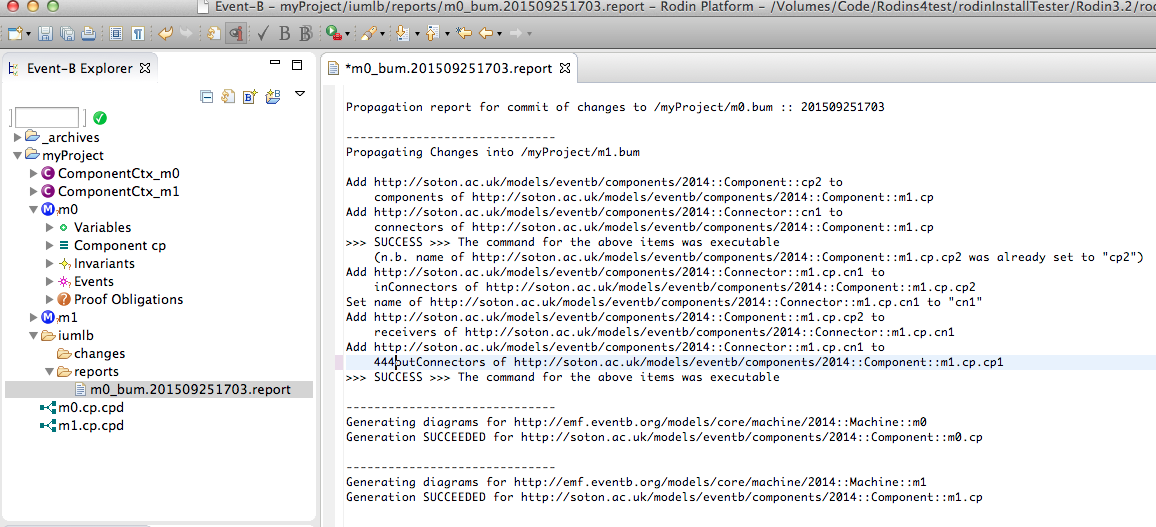
\includegraphics[width=1\textwidth]{figures/image67.png}
  \fi
  \caption{Reports Produced by Refactoring}
  \label{fig:ReportsProducedByRefactoring}
\end{figure} 

%%% Local Variables:
%%% mode: latex
%%% TeX-master: "component_diagrams-user_manual"
%%% End:


\end{document}

%%% Local Variables:
%%% mode: latex
%%% TeX-master: t
%%% End:
